\documentclass[12pt]{article}

\usepackage{amsmath, amssymb}
\usepackage{multicol}

\usepackage[margin=.5in]{geometry}

\pagestyle{empty} %% Suppress page numbers
\setlength\parindent{0pt} %% Supress indentation

\usepackage{listings}
\usepackage{color}

\definecolor{dkgreen}{rgb}{0,0.6,0}
\definecolor{gray}{rgb}{0.5,0.5,0.5}
\definecolor{mauve}{rgb}{0.58,0,0.82}

\lstset{frame=tb,
	language=Python, %% Change default language in the middle of document with \lstset{language=Java}
	belowskip=3mm,
	showstringspaces=false,
	columns=flexible,
	basicstyle={\small\ttfamily},
	numbers=none,
	numberstyle=\tiny\color{gray},
	keywordstyle=\color{blue},
	commentstyle=\color{dkgreen},
	stringstyle=\color{mauve},
	breaklines=true,
	breakatwhitespace=true,
	tabsize=3
}

\usepackage{tikz}

\begin{document}

\section{Trees}
\subsection{Binary Trees}
A binary tree is made up of nodes with left and right children. For these notes, we can assume the structure is implemented via something like the following, very minimal, \verb|Node| class:

\begin{lstlisting}
	class Node:
	
		def __init__(self, value = None):
			self.left  = None
			self.right = None
			self.value = value
\end{lstlisting}

\subsubsection*{Binary Tree Traversal}
Building a tree:
\begin{lstlisting}
	# Creating the tree nodes
	root = Node(A)
	root.left = Node(B)
	root.right = Node(C)
	root.left.left = Node(D)
	root.left.right = Node(E)
	root.right.left = Node(F)
	root.left.right = Node(G)
\end{lstlisting}
\begin{center}
	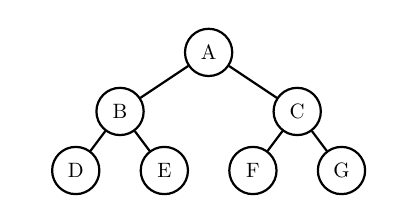
\begin{tikzpicture}[
		scale = .75, transform shape, thick,
		every node/.style = {draw, circle, minimum size = 8mm},
		grow = down,  % alignment of characters
		level 1/.style = {sibling distance=3cm},
		level 2/.style = {sibling distance=1.5cm}, 
		level 3/.style = {sibling distance=1cm}, 
		level distance = 1cm
		]
		\node (A){A}
		child { node (B) {B}			
			child { node  (D) {D}}
			child { node (E) {E}}
		}
		child { node (C) {C}
			child { node (F) {F}}
			child { node (G) {G}}
		};
		% Labels
		\begin{scope}[nodes = {draw = none}]
			
			\path (A) -- (B) node [left]  {};
			\path (A) -- (C) node [right] {};
			\path (B) -- (D) node [left] {};
			\path (B) -- (E) node [right]  {};
			\path (C) -- (F) node [left] {};
			\path (C) -- (G) node [right] {};
		\end{scope}
	\end{tikzpicture}
\end{center}

Here are three common algorithms for traversing a tree:
\begin{itemize}
	\item \textbf{In-Order}: Traverse left sub-tree, to the root, to the right sub-tree
		\subitem Result: D,B,E,A,F,C,G
		\subitem Code:
		\begin{lstlisting}
			# Function to perform inorder traversal
			def inorderTraversal(root):
				# Base case: if the current node is null, return
				if root is None:
					return None
				# Recur on the left subtree
				inorderTraversal(root.left)
				# Do whatever you want with the visited nodes...
				print(root.data)
				# Recur on the right subtree
				inorderTraversal(root.right)
		\end{lstlisting}
	\item \textbf{Pre-order}: Traverse from the root, to the left sub-tree, to the right sub-tree
		\subitem Result: A,B,D,E,C,F,G
		\subitem Code:
		\begin{lstlisting}
			def preorderTraversal(root):
				if root is None:
					return None
				print(root.data)
				preorderTraversal(root.left)
				preorderTraversal(root.right)
		\end{lstlisting}
	\item \textbf{Post-order}: Traverse from the left sub-tree, to the right sub-tree, to the root
		\subitem Result: D,E,B,F,G,C,A
		\subitem Code:
		\begin{lstlisting}			
			def postorderTraversal(root):
			if root is None:
				return None			
			postorderTraversal(root.left)
			postorderTraversal(root.right)
			print(root.data)
		\end{lstlisting}
\end{itemize}

%% TODO:
%
% Priority queues and heaps
% Self balancing binary search trees
%
% Sorting algorithms

\end{document}